%\PassOptionsToPackage{demo}{graphicx}
\PassOptionsToPackage{table}{xcolor}
\documentclass[portrait,final,a0paper,fontscale=0.310]{baposter}
\usepackage[utf8]{inputenc}
\usepackage[english]{babel}
\usepackage[T1]{fontenc}

\usepackage{relsize}
%\usepackage[breaklinks=true]{hyperref}% hyperref links are displaced with baposter because of the font scale 
\usepackage{url}
\usepackage{graphicx}
\usepackage{multicol}
\usepackage{siunitx}
\usepackage{booktabs}
\usepackage{tabulary}
\usepackage{cleveref}

\usepackage{listings}
\lstset{
 columns=fullflexible,
%  frame=single,
 breaklines=true,
 breakatwhitespace=true,
% basicstyle=\ttfamily
%  postbreak=\mbox{\textcolor{red}{$\hookrightarrow$}\space},
}
\lstset{language=SQL,morekeywords={minus,ask,bb,meta,rdfs}}

%\usepackage{times}
%\usepackage{helvet}
%\usepackage{bookman}
\usepackage{palatino}

\newcommand{\captionfont}{\footnotesize}
\usepackage[font=small,labelfont=bf]{caption}

%%%%%%%%%%%%%%%%%%%%%%%%%%%%%%%%%%%%%%%%%%%%%%%%%%%%%%%%%%%%%%%%%%%%%%%%%%%%%%%%
% Multicol Settings
%%%%%%%%%%%%%%%%%%%%%%%%%%%%%%%%%%%%%%%%%%%%%%%%%%%%%%%%%%%%%%%%%%%%%%%%%%%%%%%%
\setlength{\columnsep}{1.5em}
\setlength{\columnseprule}{0mm}

%%%%%%%%%%%%%%%%%%%%%%%%%%%%%%%%%%%%%%%%%%%%%%%%%%%%%%%%%%%%%%%%%%%%%%%%%%%%%%%%
% Save space in lists. Use this after the opening of the list
%%%%%%%%%%%%%%%%%%%%%%%%%%%%%%%%%%%%%%%%%%%%%%%%%%%%%%%%%%%%%%%%%%%%%%%%%%%%%%%%
\newcommand{\compresslist}{%
\setlength{\itemsep}{1pt}%
\setlength{\parskip}{0pt}%
\setlength{\parsep}{0pt}%
}

%%%%%%%%%%%%%%%%%%%%%%%%%%%%%%%%%%%%%%%%%%%%%%%%%%%%%%%%%%%%%%%%%%%%%%%%%%%%%%
%%% Begin of Document
%%%%%%%%%%%%%%%%%%%%%%%%%%%%%%%%%%%%%%%%%%%%%%%%%%%%%%%%%%%%%%%%%%%%%%%%%%%%%%

\begin{document}

%%%%%%%%%%%%%%%%%%%%%%%%%%%%%%%%%%%%%%%%%%%%%%%%%%%%%%%%%%%%%%%%%%%%%%%%%%%%%%
%%% Here starts the poster
%%%---------------------------------------------------------------------------
%%% Format it to your taste with the options
%%%%%%%%%%%%%%%%%%%%%%%%%%%%%%%%%%%%%%%%%%%%%%%%%%%%%%%%%%%%%%%%%%%%%%%%%%%%%%
% Define some colors

% Corporate design colors of the medical faculty of the Uni of Leipzig, new design of 2018
\definecolor{mediblue}{RGB}{0,138,201}
\definecolor{mixblue}{RGB}{0,167,214}
\definecolor{aquamarine}{RGB}{138,194,209}
%\definecolor{lowertriangle}{RGB}{9,65,81}

%%
\begin{poster}%
  % Poster Options
  {
  columns=2,
  % Show grid to help with alignment
  grid=true,
  % Column spacing
  colspacing=1em,
  % Color style
  bgColorOne=white,
  bgColorTwo=white,
  borderColor=mediblue,
  headerColorOne=mediblue,
  headerColorTwo=mediblue,
  headerFontColor=white,
  boxColorOne=white,
  boxColorTwo=mediblue,
  % Format of textbox
  textborder=roundedleft,
  % Format of text header
  eyecatcher=true,
  headerborder=closed,
  headerheight=0.12\textheight,
%  textfont=\sc, An example of changing the text font
  headershape=roundedright,
  headershade=shadelr,
  headerfont=\Large\bf\textsc, %Sans Serif
  textfont={\setlength{\parindent}{1.5em}},
  boxshade=plain,
%  background=shade-tb,
  background=plain,
  linewidth=2pt
  }
  % Eye Catcher
  {
\includegraphics[width=25em]{img/medfak.pdf}} 
  % Title
  {\bf\textsc{Linked Open Data about Management of Health Information Systems}\vspace{0.5em}
  }
  % Authors
  {\textsc{Konrad Höffner, Franziska Jahn, Anna Lörke, Thomas Pause, Birgit Schneider,Elske
  Ammenwerth, Alfred Winter}}
  % University logo
  {% The makebox allows the title to flow into the logo, this is a hack because of the L shaped logo.
    %
\includegraphics[height=9.0em]{img/medfak.pdf}
  }

%%%%%%%%%%%%%%%%%%%%%%%%%%%%%%%%%%%%%%%%%%%%%%%%%%%%%%%%%%%%%%%%%%%%%%%%%%%%%%
%%% Now define the boxes that make up the poster
%%%---------------------------------------------------------------------------
%%% Each box has a name and can be placed absolutely or relatively.
%%% The only inconvenience is that you can only specify a relative position 
%%% towards an already declared box. So if you have a box attached to the 
%%% bottom, one to the top and a third one which should be in between, you 
%%% have to specify the top and bottom boxes before you specify the middle 
%%% box.
%%%%%%%%%%%%%%%%%%%%%%%%%%%%%%%%%%%%%%%%%%%%%%%%%%%%%%%%%%%%%%%%%%%%%%%%%%%%%%
    %
    % A coloured circle useful as a bullet with an adjustably strong filling
    \newcommand{\colouredcircle}{%
      \tikz{\useasboundingbox (-0.2em,-0.32em) rectangle(0.2em,0.32em); \draw[draw=black,fill=imiseblue,line width=0.03em] (0,0) circle(0.18em);}}

%%%%%%%%%%%%%%%%%%%%%%%%%%%%%%%%%%%%%%%%%%%%%%%%%%%%%%%%%%%%%%%%%%%%%%%%%%%%%%
\begin{posterbox}[name=background,column=0,row=0]{Background}

\begin{minipage}{\linewidth}
\centering
\captionof{figure}{The SNIK Meta Model}
\label{fig:metamodel}
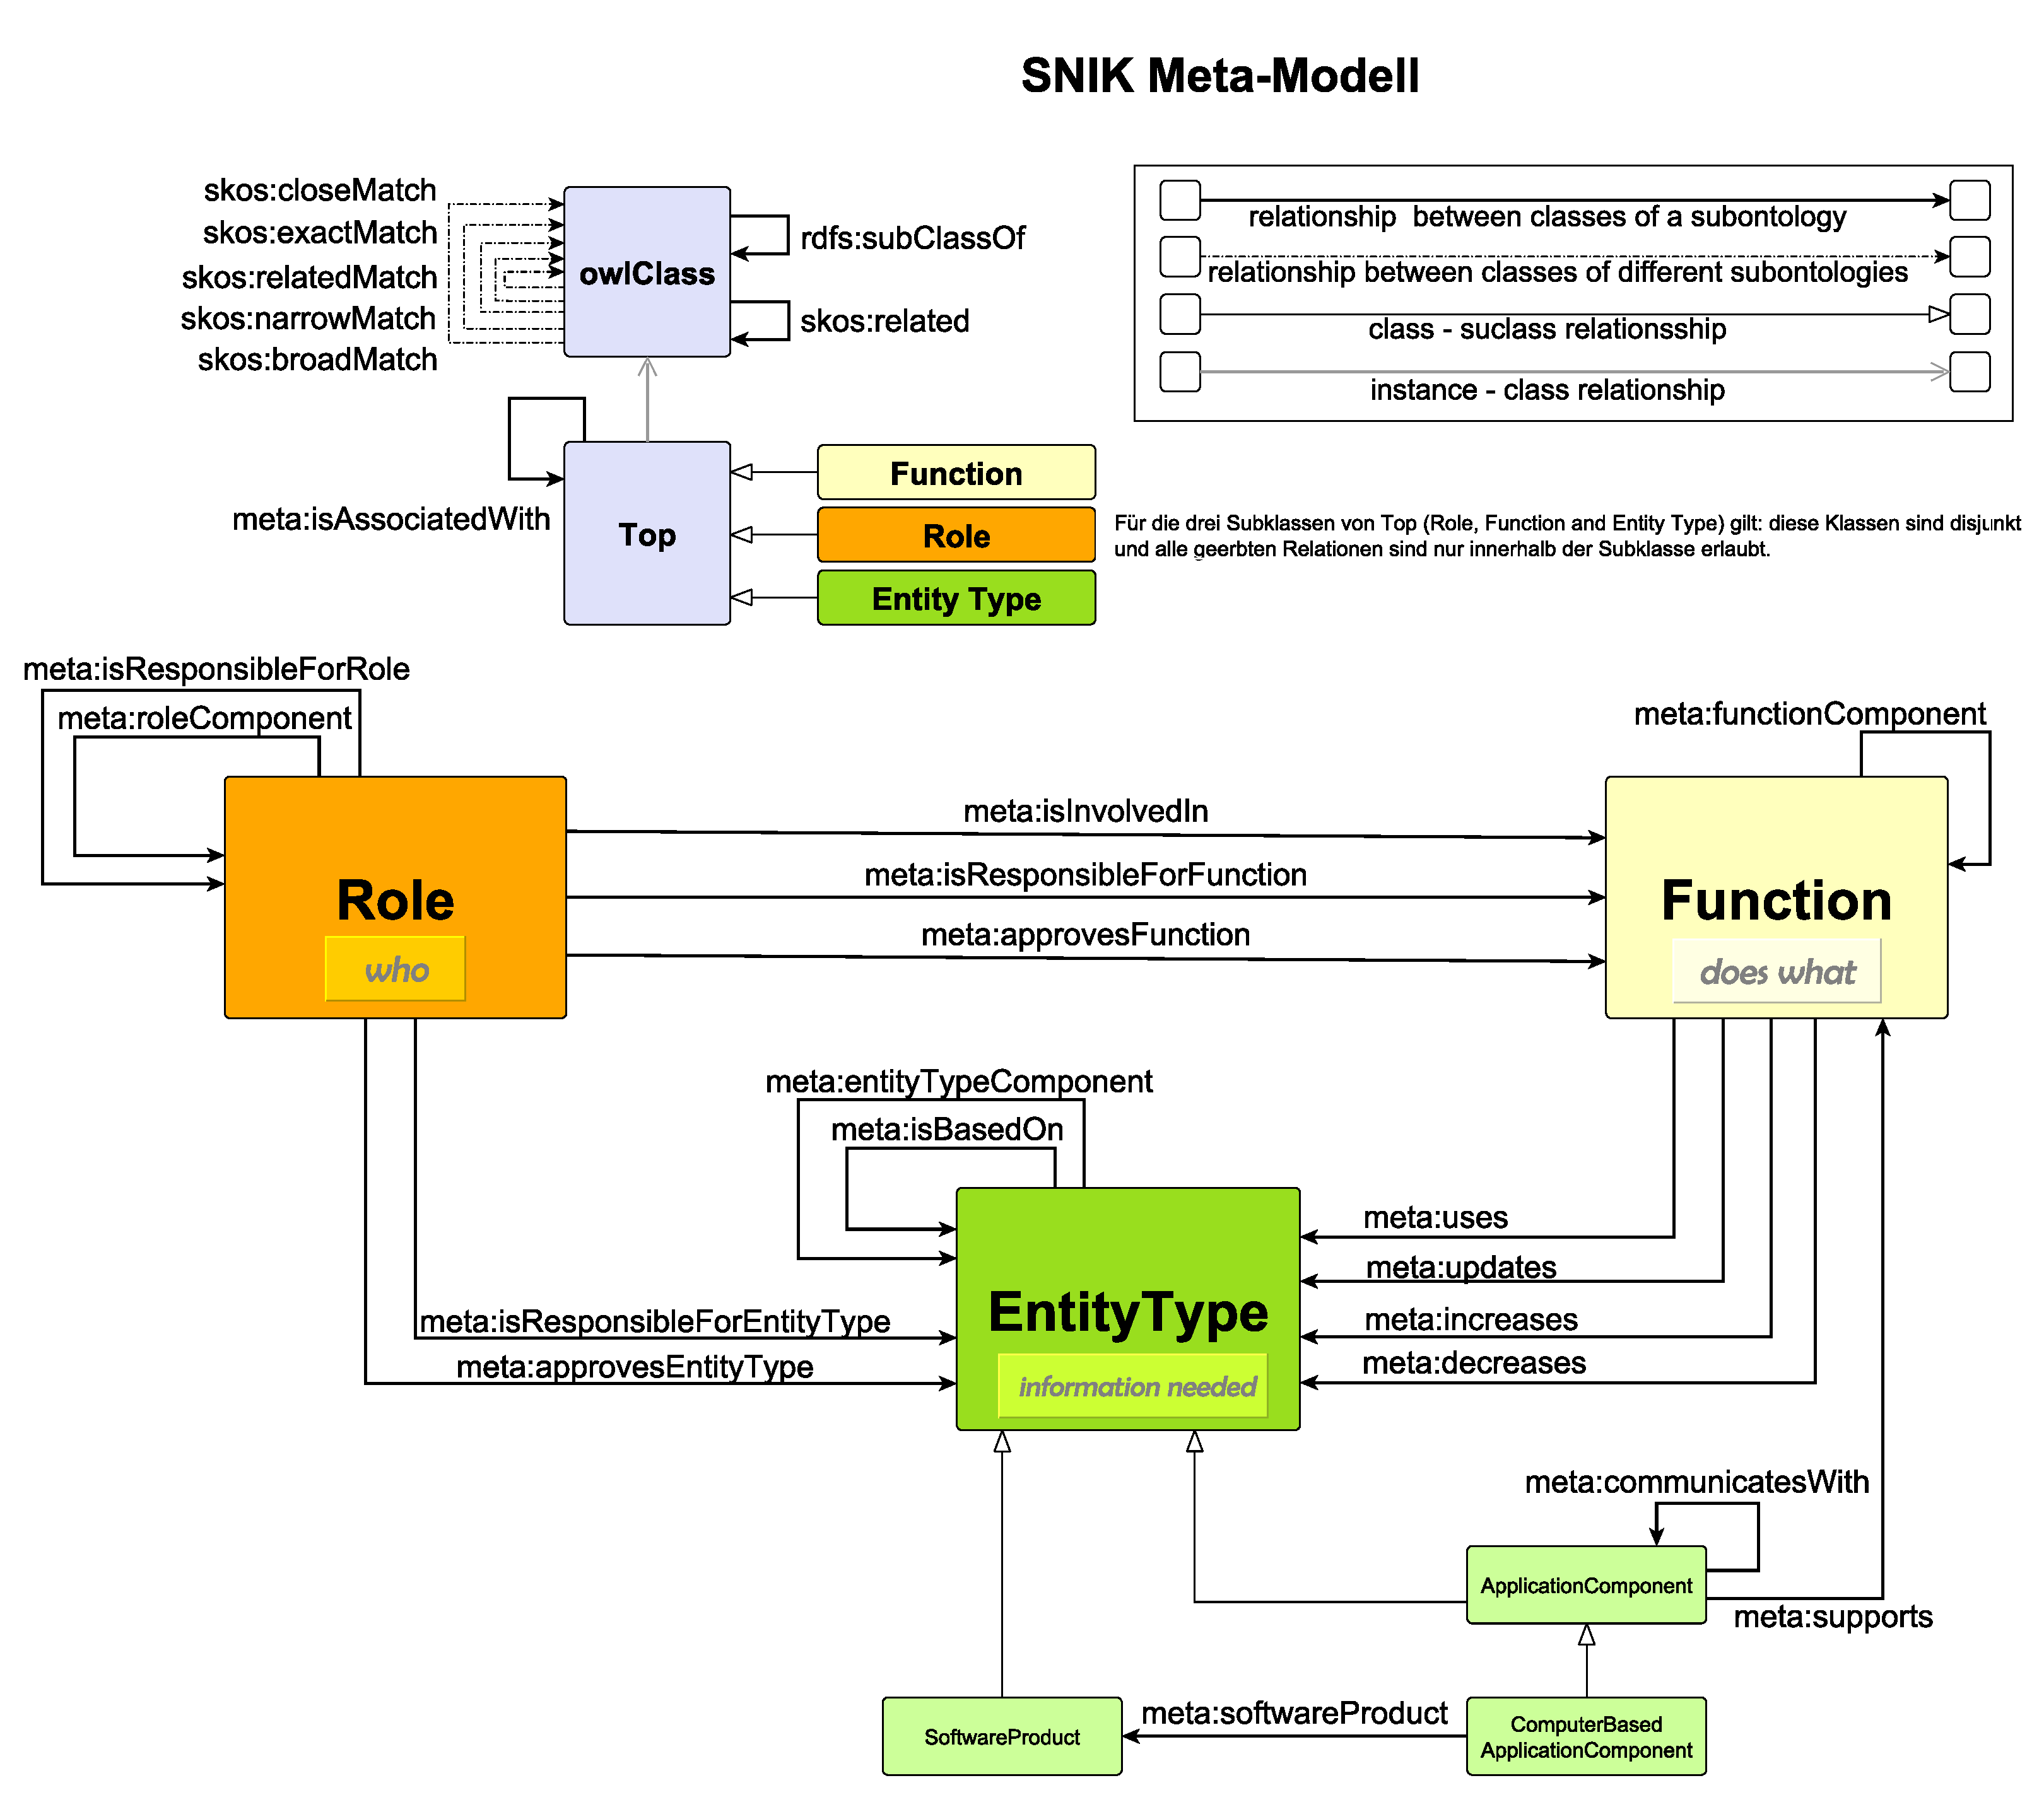
\includegraphics[width=\columnwidth]{img/metamodel.pdf}
\end{minipage}
The Semantic Network of Information Management in Hospitals (SNIK) is an OWL 2 DL ontology with a modular architecture:
The Meta Model provides a common vocabulary for the domain of HIS management and thus defines, which superclasses and relations can be used, see \cref{fig:metamodel}.
Five subontologies are built upon the meta model: bb,ob,he,ciox,it4it.
%The SNIK project uses Ontologies and Linked Data technologies to  
%Management of hospital information systems (HIS) is an exceptionally challenging task.
%There is an enormous amount of frameworks, textbooks and articles describing the scope from the perspective of medical informatics.
%However, the disciplines of business informatics and information systems (IS) provide an even broader view on information systems and their management.
%How can knowledge on HIS management be made easily and freely available and how can this knowledge be combined with other knowledge in biomedical and health informatics and in other disciplines?
\vspace{0.3em}
\end{posterbox}
%%%%%%%%%%%%%%%%%%%%%%%%%%%%%%%%%%%%%%%%%%%%%%%%%%%%%%%%%%%%%%%%%%%%%%%%%%%%%%
\begin{posterbox}[name=results,below=background]{RDF Browser}
%We present several interfaces of SNIK that are useful for researchers practitioners and students, depending on their objectives and their semantic web skills.
%We show that those interfaces can benefit teaching, system analysis and integration.
\end{posterbox}
%%%%%%%%%%%%%%%%%%%%%%%%%%%%%%%%%%%%%%%%%%%%%%%%%%%%%%%%%%%%%%%%%%%%%%%%%%%%%%
\begin{posterbox}[name=results,below=background]{Results}
%We present several interfaces of SNIK that are useful for researchers practitioners and students, depending on their objectives and their semantic web skills.
%We show that those interfaces can benefit teaching, system analysis and integration.

\end{posterbox}
%%%%%%%%%%%%%%%%%%%%%%%%%%%%%%%%%%%%%%%%%%%%%%%%%%%%%%%%%%%%%%%%%%%%%%%%%%%%%%
\begin{posterbox}[name=references,column=0,below=results]{References}
    \smaller
    \bibliographystyle{ieee}
    \renewcommand{\section}[2]{\vskip 0.05em}
      \begin{thebibliography}{1}\itemsep=-0.01em
      \setlength{\baselineskip}{0.4em}
      \bibitem{amberg11:graphtrack}
        B.~Amberg, T. Vetter.
        \newblock {GraphTrack}: {F}ast and {G}lobally {O}ptimal {T}racking in {V}ideos
        \newblock In {\em CVPR '11}
      \bibitem{awf:tracking}
        A.~Buchanan and A.~Fitzgibbon.
        \newblock {I}nteractive {F}eature {T}racking using {K-D} {T}rees and {D}ynamic {P}rogramming.
        \newblock In {\em CVPR '06}
      \end{thebibliography}
   \vspace{0.3em}
  \end{posterbox}
%%%%%%%%%%%%%%%%%%%%%%%%%%%%%%%%%%%%%%%%%%%%%%%%%%%%%%%%%%%%%%%%%%%%%%%%%%%%%%
\begin{posterbox}[name=snikgraph,column=1,row=0]{SNIK Graph}
\indent
The most intuitive interface to SNIK is the SNIK Graph visualization, which is based on the Cytoscape.js browser graph library.
SNIK Graph queries the list of classes and their relations from the SPARQL endpoint and transforms them into nodes and edges of the graph.
Exploration options like the “spider worm”, which consists of the shortest path between a start node and an end node together with the end node’s neighbourhood, illustrate the context of a concept.
\vspace{0.3em}
  \end{posterbox}
%%%%%%%%%%%%%%%%%%%%%%%%%%%%%%%%%%%%%%%%%%%%%%%%%%%%%%%%%%%%%%%%%%%%%%%%%%%%%%
\begin{posterbox}[name=sparql,column=1,above=bottom]{SPARQL}
\noindent
Public access to the meta model and the subontologies via SPARQL queries:

\vspace{1em}
{
\rowcolors{0}{mediblue!20}{white}
\centering
\begin{tabular*}{\columnwidth}{l}
Which components of a healthcare network are not healthcare institutions?\\
\begin{lstlisting}
SELECT ?x {bb:HealthCareNetwork meta:entityTypeComponent ?x.
  MINUS {?x rdfs:subClassOf* bb:HealthCareInstitution.}}
\end{lstlisting}\\
%bb:GovernmentalAuthority\\

How many functions is the CIO responsible for?\\
\begin{lstlisting}
SELECT COUNT(?f) {bb:ChiefInformationOfficer meta:isResponsibleForFunction ?f.}
\end{lstlisting}\\
%15\\

Do transinstitutional health information systems support telemicroscopy?\\
\begin{lstlisting}
ASK {bb:TransinstitutionalHealthInformationSystem meta:supports bb:Telemicroscopy.}
\end{lstlisting}
\end{tabular*}
%True
}
\vspace{0.0em}
\end{posterbox}
%%%%%%%%%%%%%%%%%%%%%%%%%%%%%%%%%%%%%%%%%%%%%%%%%%%%%%%%%%%%%%%%%%%%%%%%%%%%%%
\begin{posterbox}[name=source,column=1,above=sparql,below=background]{Details}
\begin{tabulary}{\columnwidth}{lL}
URL		&\url{http://www.snik.eu/ontology}\\
Version		&2018-10-10, 0.4.1\\
License		&CC BY-NC-SA 4.0\\
SPARQL Endpoint	&\url{http://www.snik.eu/sparql}\\
Subontologies	&\url{http://www.snik.eu/ontology/bb}\\
		&\url{http://www.snik.eu/ontology/ciox,}\\
		&\url{http://www.snik.eu/ontology/ob}\\
		&\url{http://www.snik.eu/ontology/he}\\
		&\url{http://www.snik.eu/ontology/it4it}\\
Visualization	&\url{http://www.snik.eu/graph}\\
RDF Browser	&\url{http://www.snik.eu/ontology}\\
RDF Dump	&\url{https://github.com/IMISE/snik-ontology/releases/download/0.4.1/snik-0.4.1-combined.nt.zip}\\
\# Triples	&\num{112747}\\
\# Classes	&\num{4729}\\
\# Properties	&\num{329}\\
\# Interlinks	&\num{713}\\
\end{tabulary}%The source code for the services is available at \url{https://github.com/imise}
\end{posterbox}
%%%%%%%%%%%%%%%%%%%%%%%%%%%%%%%%%%%%%%%%%%%%%%%%%%%%%%%%%%%%%%%%%%%%%%%%%%%%%%
\end{poster}
\end{document}

